\subsection{Forecasting Future Flow}
\label{sec:futureflow}

\begin{figure*}[tbh]
	\centering
	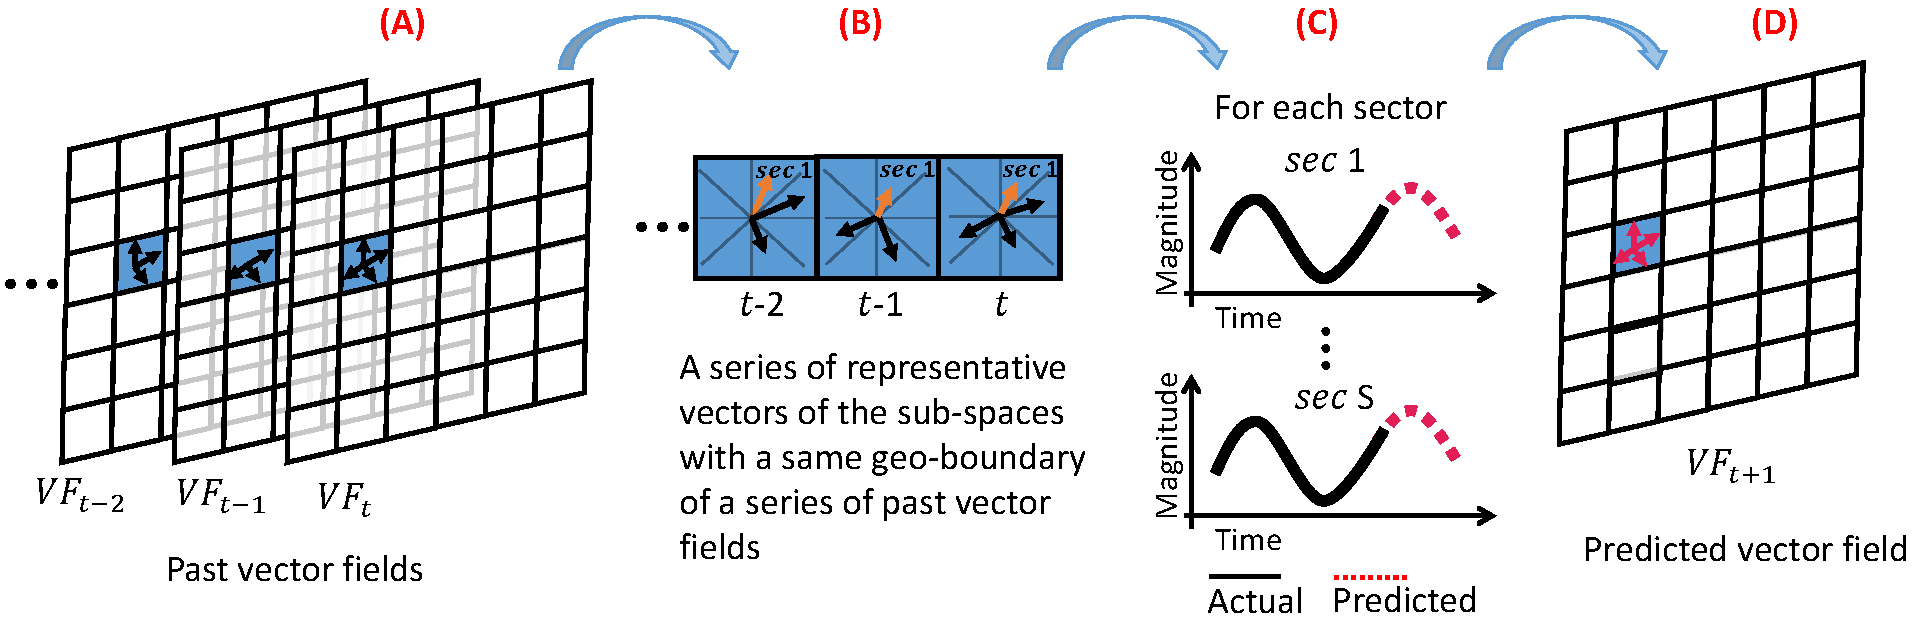
\includegraphics[width=1.0\linewidth]{forecasting_v2}
	\caption{The process of multi-vector field prediction. 
	%We generate a series of the past vector fields (A). a set of smoothed representative vectors for each individual sub-space and A time series vectors are considered to generate a series of representative vectors for each sub-space as shown in (B). (C) for each sector, magnitudes are computed based on STL to have final representative vectors in each space (D).  
	}
	\label{fig:forecasting}
	%\vspace{-0.7cm}
\end{figure*} 

To forecast directional density using historical vector-based crowd data, we apply seasonal trend decomposition based on LOESS technique~\cite{Cleveland:1990:SAS} over the entire space. %on each sub-space. % in order to compute history-based representative vectors for the entire space. 
%We forecast the future flow of a space based on the calculated historical directional density for the sub-spaces of the space utilizing a seasonal trend analysis method~\cite{Cleveland:1990:SAS}.
%Our model forecast the future representative vectors for each sectors of each sub-space separately.
%We then combine the forecasted representative vectors resulted in the future flow as a whole for the entire space.
Figure~\ref{fig:forecasting} illustrates the overall process of our forecasting method.
%In our predictive scheme, each data of the directional distribution is treated as a separate time series variable.
%\textbf{Creating past vector fields:}
For a given geo-location boundary~$\Omega$ and a past time window $t$, 
%(e.g., by day, week) 
we first prepare 
the geospace with the trajectory data (Figure~\ref{fig:forecasting}~(A)).
Next, we fragment the geospace~$\Omega$ into sub-spaces and compute a set of smoothed representative vectors for each individual sub-space using the methodology described in Sections~\ref{sec:discretization} and~\ref{sec:smoothing}.
%As described in Section~\ref{sec:discretization} and ~\ref{sec:smoothing}, then we calculate a set of smoothed representative vectors for each individual sub-space of the space.
%Compared to conventional methods where one vector is assigned to a sub-space for generating a vector field,
%Conventionally, one vector is assigned to a sub-space for generating a vector field.
As discussed previously, we 
%we instead 
calculate a set of representative vectors $\vec{V_k}$ for each sub-space in order to create a multi-vector field (i.e., we calculate representative vectors for each sector of the sub-space (Figure~\ref{fig:forecasting}~(A))).
This is shown in Figure~\ref{fig:forecasting}~(A). % called a multi-vector field.
In our approach, we define these vector fields for the given time window $t$ as 
$VF_t = \left\{\mathcal{M}_{sp_{i}}, \enspace sp_{i} \in \Omega \right\}$, 
where $\mathcal{M}_{sp_{i}}$ is a set of smoothed representative vectors for sub-space $sp_i$.
%for a time window $t$ (e.g., a day), such a vector field is defined as $VF_t = \left\{\mathcal{M}_{sp_{i}}, \enspace sp_{i} \in \Omega \right\}$, where $\mathcal{M}_{sp_{i}}$ is a set of smoothed representative vectors for a sub-space $sp_i$.
%$\Delta{duration}$ is the time duration of the time window (e.g., 3 hours),
This process is repeated for each sub-space in geospace for a given time step, and then over time for the entire time window $t$ (Figure~\ref{fig:forecasting}~(B)). 
%We repeatedly shift the time window $t$ backward and create multi-vector fields for time window $t$ (Figure~\ref{fig:forecasting} (A)) [ISN'T THIS REPETITIVE?].
%\textbf{Extracting series of representative vector sets:}
%Next, we extract a series of $\mathcal{M}_{sp_{i}}$ for each sub-space 
%with a same geo-boundary 
%from the historical multi-vector fields (Figure~\ref{fig:forecasting} (B)).
%\textbf{Preparing time series and forecasting:}
Next, we generate a time series of the \textit{magnitude} values of the representative vectors of the series of $\mathcal{M}_{sp_{i}}$ for each sector of the sub-space (Figure~\ref{fig:forecasting}~(C)).
%that result in $S$ (the number of divided sectors) time series (See Figure~\ref{fig:forecasting} (C)) \textcolor{red}{[???TOO LONG].}
%For a sub-space $sp_i$, 
This time series is defined as:
\begin{equation}
Y_k = \left\{M(\vec{V_k}): \vec{V_k} \in \mathcal{M}_{sp_{i}}, \mathcal{M}_{sp_{i}} \in VF_t, t \in T\right\}, k = \left\{1, \cdots, S\right\}
\end{equation}
Here, $T$ is the time range of observed historical data. % [ARE THE REST OF THE TERMS DEFINED PREVIOUSLY?].

In order to model the time series $Y_k$ and forecast for the future value, we employ the seasonal-trend decomposition technique (STL) described in~\cite{Maciejewski:2011:Forecasting, Malik:2014:Proactive}. 
The technique is based on a locally weighted regression (loess) methodology (STL)~\cite{Cleveland:1990:SAS}.
For each sub-space, we predict the future magnitude value of the representative vector (Figure~\ref{fig:forecasting}~(C)).
%resulted in a set of the predicted representative vectors for the sub-space (See Figure~\ref{fig:forecasting} (D)). \textcolor{red}{[???]}
Finally, we repeat this process for every single sub-space and their corresponding sectors, and generate the future multi-vector field $VF_{t+1}$ (Figure~\ref{fig:forecasting}~(D)).

%Our model repeat to create such vector field a space for a past time interval.
%then prepares a series of such vector fields for a series of the corresponding past time intervals.
%for a certain past period of time frames,

%\begin{enumerate}
	%\item Creating a series of VFs for a certain past period of time frames,
	%\item Extracting a series of vectors from the cells with a same coordinate from the series of VFs,
	%\item Generating two time series, directions and magnitudes, of the series of vectors,
	%\item Applying a temporal prediction method to the two time series for predicting the direction and the magnitude of the future \item vector of the coordinate, and
	%\item Repeating the same procedure on each coordinate to create the future VFs.
%\end{enumerate}


%Forecasting analysis of multiple vector fields using STL
